\chapter{Movimiento parabólico:} 
 
\textit{``¿Por qué las cosas son como son y no de otra manera?''} \textbf{Johannes Kepler}
\vspace{1.0cm}  
 
También llamado tiro de proyectiles, corresponde al movimiento de un proyectil en el campo gravitatorio y que cuya  trayectoria 
es 
una parábola.
 
\begin{figure}[ht]
 \centering
 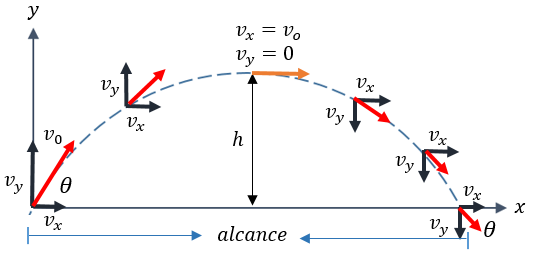
\includegraphics[scale=0.6]{images/movimiento_parabolico.png}
 % cinematica.png: 0x0 px, 300dpi, 0.00x0.00 cm, bb=
 \caption{Ilustración del movimiento parabólico.}\label{movparabola}
\end{figure}   

Para el análisis de este movimiento se lo considera como la composición de dos movimientos: horizontal (respecto al eje x) y 
vertical (respecto al eje y).\\

Antes de analizar estos submovimientos hay que considerar que el móvil inicia su movimiento con una velocidad inicial $\vec{v_0}$ 
que hace un ángulo $\theta$ (ángulo de tiro) con la horizontal referenciada con el eje x positivo. Así, resulta conveniente 
encontrar las componentes de esta velocidad en cada eje cartesiano, y estas son:

\begin{equation}
 \vec{v_{0x}}=\vec{v_0}cos(\theta)
\end{equation}

\begin{equation}
 \vec{v_{0y}}=\vec{v_0}sen(\theta)
\end{equation}

\textbf{Movimiento horizontal:}\\

Este movimiento se refiere al movimiento de la proyección del cuerpo en el eje $x$, en este eje la velocidad es constante, es 
decir, $\vec{v_{0x}} =  \text{constante} = v_x$ y por tanto el movimiento en este eje es MRU, y por tanto la ecuación de 
movimiento es:

\begin{equation}
 x = v_{0x}t=v_x \Delta t
\end{equation}

A la distancia máxima en el eje $x$ que la proyección del cuerpo logra moverse se la denomina alcance máximo ($x_{max}$). Y al 
tiempo que demoró en cubrir esa distancia se la llama tiempo de vuelo ($t_v$), con lo cual alcance máximo es:

\begin{equation}
 x_{max} =  v_x t_v
\end{equation}

\textbf{Movimiento vertical:}\\

Este es el movimiento correspondiente en el eje $y$, en este movimiento se considera la acción de la gravedad ($g$), además, hay 
que distinguir que el movimiento se divide en dos etapas: la primera en la que el cuerpo sube con una velocidad inicial $v_{0y} = 
 v_0 sen(\theta)$ y llega a una altura máxima $h_{max}$ donde el cuerpo tiene una velocidad en $y$ de 0 (en esta etapa se ha 
realizado un lanzamiento vertical), luego en el cuerpo cae con una velocidad inicial en $y$ de cero así que cae realizando una 
caída libre.\\

Entonces la velocidad del cuerpo en cualquier instante es:

\begin{equation}
 \vec{v} = \vec{v_x} + \vec{v_y}\quad \text{cuyo módulo es:} \quad v = \sqrt{v_x^2+v_y^2}
\end{equation}

Debido a la simetría del movimiento en el eje $y$ es notorio que el tiempo de vuelo es el doble del tiempo de subida como el 
tiempo de bajada.

\begin{equation}
 t_v = 2t_s =2t_b
\end{equation}

Además, que las ecuaciones de movimiento en el eje de las $y$ son las de lanzamiento vertical y caída libre respectivamente:

\begin{equation}
 v_{fy} = v_{0y} + gt
\end{equation}

\begin{equation}
 v_{fy}^2 = v_{0y}^2 + 2gh
\end{equation}\label{dos}

\begin{equation}
 h =(\frac{v_{fy}+v_{oy}}{2})t
\end{equation}

\begin{equation}
 h = v_{oy}t + \frac{1}{2}gt^2
\end{equation}

Y así por tanto para encontrar por ejemplo la altura mámixa se utiliza la ecuación (\ref{dos}) sabiendo que la $v_{fy} = 0$, así 
que:

\begin{equation}
 h_{max} = -\frac{v_0^2sen^2(\theta)}{2g}
\end{equation}

\section{Problemas de movimiento parabólico}

\begin{enumerate}

 \item Un soldado acostado en el suelo lanza una granada con velocidad inicial de 25 m/s, y un ángulo de elevación de
 $53^\circ$. Despues de que tiempo escuchará el estallido. Velocidad del sonido: 340m/s.
 
 \item Se dispara una flecha a 25 m/s y a $30^\circ$ con la horizontal,
 para dar en un árbol que está a 30 metros de distancia. 
Determinar: a) la altura a la que se elevará
 la flecha,  b) el ángulo que formarán la
 flecha con el árbol, y c) el tiempo que 
tarda la flecha hasta dar con el árbol. 


\item Un jugador de Fútbol Americano patea el balón con una velocidad de 30 m/s, y éste mismo
 lleva un ángulo de elevación de 
$45^\circ
$ respecto a la horizontal. Calcule; a) altura, b) alcance, y c) tiempo que
 permanece en el aire.

\item  Un proyectil es lanzado de modo que su alcance máximo
 es de 44 m. Sabiendo que el ángulo de tiro es de $45^\circ$, 
averigua la velocidad inicial del
 lanzamiento. 

\item Se dispara un proyectil con una velocidad inicial de 50 m/s
 y un ángulo de $25^\circ$, por encima de la horizontal. 
Calcular la velocidad del proyectil después de
 los 6s.

\item Se dispara un proyectil con una velocidad inicial de 60 m/s y un ángulo de $30^\circ
$, por encima de
 la horizontal. 
Calcular: a) Posición y velocidad después de los 6s, b) tiempo para alcanzar la altura máxima
 y c) el  alcance horizontal.

\item  Un proyectil es lanzado de modo que su alcance máximo
 es de 55 m. Sabiendo que el ángulo de tiro es de $45^\circ$, 
averigua la velocidad inicial del
 lanzamiento. 

\item Dos personas, A y B, se encuentran en las ventanas de dos edificios ubicados uno frente a
 otro, en los lados opuestos de 
una calle. Los edificios est´an separados entre sí 10 m y las alturas de las
 ventanas respecto al piso son 15 m para A y 20 m 
para B. Si B lanza, hacia la derecha, un globo con agua
 con la intención de impactar a A y la rapidez inicial del globo es de 
10 m/s, calcule: a) el ángulo de disparo
 respecto a la horizontal, y b) el vector velocidad del proyectil el momento del impacto.

\end{enumerate}
